\documentclass[]{beamer}
\usepackage{xmpmulti}
\usepackage{psfrag}
\usepackage{xcolor}
\newcommand{\owner}{\mathcal{O}}
\newcommand{\manager}{\mathcal{M}}

\mode<presentation>
{\usetheme{Boadilla}  % very plain
}

\usepackage{xcolor}

\usepackage{amssymb,amsmath,amsthm}
\usepackage{boxedminipage}

\usepackage{tikz}
\usetikzlibrary{snakes}
\usetikzlibrary{backgrounds} 
\usepgflibrary{shapes.geometric}
\usepgflibrary{shapes.misc}
\usepackage{pgfmath}


\newcommand{\view}{{\mathsf{view}}}
\newcommand{\DS}{{\mathsf{DS}}}
\newcommand{\emm}{{\mathsf{eMM}}}
\newcommand{\mm}{{\mathsf{MM}}}
\newcommand{\aep}{{\mathsf{aep}}}
\newcommand{\gep}{{\mathsf{gep}}}
\newcommand{\Dist}{{\mathsf{Dist}}}
\newcommand{\Hard}{{\mathsf{Hard}}}
\newcommand{\key}{\mathtt{key}}
\newcommand{\GetMM}{\mathsf{Get}}
\newcommand{\AddMM}{\mathsf{Add}}

\newcommand{\vals}{\vec{\mathtt{v}}}
\newcommand{\val}{{\mathtt{v}}}
\newcommand{\op}{{\mathtt{op}}}

\newcommand{\calA}{\mathcal{A}}
\newcommand{\calL}{\mathcal{L}}
\newcommand{\lQ}{\calL^G}
\newcommand{\lU}{\calL^A}

\setbeamercolor{uppercol}{fg=teal,bg=lightgray}%
\setbeamercolor{lowercol}{fg=olive,bg=lightgray!50}%

\newcommand{\aaa}{\mathsf{a}}
\renewcommand{\ggg}{\mathsf{g}}

\title[]{Leakage in the Cell Probe Model \\ Lower Bounds for Response Hiding Encrypted Multi-Maps}

\author{Giuseppe Persiano}

\institute[UNISA]{%
Universit\`a di Salerno\\ \qquad \\
}

\date[June 2019]{June, 2019}

\begin{document}

\newcommand{\zu}{\{0,1\}}
\newcommand{\ignore}[1]{}

\begin{frame}
  \titlepage

Describing joint work with:

Sarvar Patel and Kevin Yeo (Google LLC)
\end{frame}




\begin{frame}
\frametitle{The Model}

\begin{block}{Cell Probe Model for a Data Structure [Yao]}
\begin{itemize}
\item Memory is a sequence of {\em\color{purple} cells} each of $\color{purple} w$ bits
\vskip .4cm
\item Accessing (reading/writing) a cell cost $1$
\vskip .4cm
\item All computation is for free
\end{itemize}
\end{block}

\vfill
Classical model used to derive lower bounds for Data Structures
\end{frame}

\begin{frame}
\frametitle{The Oblivious Model}
\begin{block}{Oblivious Cell Probe Model [Larsen+Nielsen '18]}
In a Client-Server setting
\begin{itemize}
\item Client outsources storage of the $\color{purple} \DS$ to an {\color{purple} \em honest-but-curios} server
\item Client performs $\color{purple} \DS$ operations $\color{purple} O=(\op_1,\ldots,\op_l)$ by accessing the Server memory
    \begin{itemize}
    \item client can read and write any {\em cell} in Server memory
    \item each cell is $w$-bit wide
    \end{itemize}
\item Client has {\color{blue} limited} private local memory
\item Server observes the access pattern and the data downloaded
    \begin{itemize}
        \item $\color{magenta} \view^{\DS}(O)=
            \left(\view^\DS(\op_1),\ldots,\view^\DS(\op_l)\right)$
    \end{itemize}
    \item {\color{blue}\bf Passive} server: performs no computation
    \item Operations are performed {\color{blue}\bf online}
    \end{itemize}
    \end{block}
    \end{frame}

    \begin{frame}
    \frametitle{Security Notion}
    \begin{definition}
    $\color{magenta}\DS$ is {\color{blue} Oblivious},
    if for every PPT machine $\calA$ and any two sequences $O$ and $O'$ of the
    {\color{red} same length}
    $$\color{blue} \left|
        \text{Prob}\left[\calA(\view^\DS(O))=1\right]
            -
        \text{Prob}\left[\calA(\view^\DS(O'))=1\right]
        \right|\leq \frac{1}{4}.$$
    \end{definition}
    \end{frame}

    \begin{frame}
    \frametitle{The array maintenance problem (a.k.a. ORAM)}
\vskip .4cm

    Two operations to maintain an $\color{magenta}n$-slot array $\color{magenta}A$
    \begin{itemize}
    \item $\color{magenta} \mathsf{Read}(i)$ returns the current value stored in $\color{magenta}A[i]$
    \item $\color{magenta} \mathsf{Write}(i,x)$ sets $\color{magenta}A[i]:=x$
    \end{itemize}

\pause

\vskip 2cm
    \begin{theorem}[Larsen+Nielsen '18]
    Expected amortized running time of an ORAM with $\color{purple}n$ $\color{purple}b$-bit slots is
    $$\color{purple} \Omega\left(
    \frac{b}{w}\cdot\log\frac{nb}{c}
                    \right)$$
    where $\color{purple} c$ is the client memory in bits.
    \end{theorem}

\pause
\alert{Online Read and Write operations with Passive Server}
\end{frame}

\begin{frame}
\frametitle{Proof strategy for ORAM lower bound [Larsen+Nielsen]}
\begin{block}{The Information Transfer Technique [P\v{a}tra\c{s}cu+Demaine]}
\begin{itemize}
\item assign probes to nodes of the {\color{red} Information Tree}
    \begin{itemize}
        \item each probe to at {\color{red} most one node}
    \end{itemize}
\vskip .6 cm 
\item show that for {\color{red} most} nodes $\color{purple} v$ there exists a
        {\color{red} hard distribution $\color{red}\mathbf{HD_v}$} on sequences of operations 
    of the {\color{red} same length} that assign lots of probes to $\color{purple}v$
    \begin{itemize}
        \item {\color{green} coding argument leveraging on {\color{red} randomness} of the entries of the array}
    \end{itemize}
\vskip .6 cm 
\item invoke {\color{red}\bf obliviousness}
    to show that for each such distribution all nodes must be assigned
the same {\color{red} high} number of probes
\end{itemize}
\end{block}
\end{frame}


\begin{frame}
\frametitle{Obliviousness}
\begin{itemize}
\item very \alert{strong} requirement
\vskip .3cm
\item it hides the type of operation
\vskip .3cm
\item it hides the parameters of the operations
\vskip .3cm
\begin{itemize}
  \item the content of the array (for $\color{magenta} \mathsf{Write}$)
  \item the slot of the operation (for $\color{magenta} \mathsf{Read}$ and $\color{magenta} \mathsf{Write}$)
\end{itemize}
\vskip .3cm
\item only number of operations is leaked
\vskip .3cm
\end{itemize}

\pause
\vfill
In several applications more information is leaked for the sake of efficiency
\end{frame}

    \begin{frame}
    \frametitle{Differential Privacy}
    \begin{definition}
    $\color{magenta}\DS$ is {\color{blue} $(\epsilon,\delta)$-DP},
    if for every PPT machine $\calA$ and any two sequences $O$ and $O'$ of the 
    {\color{red} same length}
    that differ for {\color{red} exactly one operation}
    $$\color{blue} 
        \text{Prob}\left[\calA(\view^\emm(O))=1\right]
        \leq e^\epsilon\cdot\text{Prob}\left[\calA(\view^\emm(O'))=1\right]+\delta
        $$
    \end{definition}
    \end{frame}

    \begin{frame}
    \frametitle{The Differentially Private RAM}
    \begin{theorem}[P+Yeo '19]
    For every $\epsilon>0$ and $\delta\leq 1/3$, the 
    expected amortized running time of a {\color{red} Differentially Private RAM} 
with $\color{purple} n$ $\color{purple} b$-bit slots is
    $$\color{purple} \Omega\left(
    \frac{b}{w}\cdot\log\frac{nb}{c}
                    \right)$$
    where $\color{purple} c$ is the client memory in bits.
    \end{theorem}

\pause
\vfill
\alert{Different proof technique}
\end{frame}

\begin{frame}
\frametitle{Leakage Cell Probe Model}

A sequence of operations $\color{magenta} O=(\op_1,\op_2,\ldots,\op_l)$
is associated with {\color{magenta} leakage $\calL(O)$}

$$\color{magenta}\calL(O)=(\calL(\op_1),\ldots,\calL(\op_l))$$

\pause

\begin{definition}
$\color{magenta}\DS$ is {\color{blue} Non-Adaptively $\color{magenta} \calL$-INDSecure},
if for every PPT machine $\calA$ and any two sequences $O$ and $O'$ such that
$\color{red}\calL(O)=\calL(O')$, 
$$\color{blue} \left|
    \text{Prob}\left[\calA(\view^\DS(O))=1\right]
        -
    \text{Prob}\left[\calA(\view^\DS(O'))=1\right]
    \right|\leq \frac{1}{4}.$$
\end{definition}
\pause
\vfill
{\color{olive} Oblivious considers leakage $\calL(O)=l$}
\end{frame}





\begin{frame}
\frametitle{Multi-Maps (MM)}
\begin{block}{Multi-Maps}
A {\color{blue} data structure} to maintain a collection of pairs $\color{purple}(\key,\vals)$,
where $\color{purple}\vals=(v_1,\ldots,v_l)$ is a tuple
\begin{enumerate}
\vskip 1cm
\item $\color{purple}\AddMM(\key,\val)$: {\em adds $\color{purple}\val$ to the tuple associated with $\color{purple}\key$}
\vskip 1cm
\item $\color{purple}\GetMM(\key)$: {\em returns the tuple associated with $\color{purple}\key$}
\end{enumerate}
\end{block}
\pause
\begin{itemize}[<+->]
\item A special case of {\color{red} Structured Encryption} [Chase-Kamara]
\item A {\color{purple} generalization} of ORAM:
    \begin{itemize}
        \item ORAM is a MM with all tuples of length 1;
    \end{itemize}
\end{itemize}
\end{frame}


\begin{frame}
\frametitle{How expensive are EMM?}

\pause
\alert{\bf It depends on the leakage function}
\vskip .2cm

\pause
If no security is sought: 
$$\color{purple}{O\left(\frac{\log\log n}{\log\log\log n}\right)}$$
    
\hfill [Beame and Fich '99]

\vskip .5cm
\pause
If only number of operations is leaked
$$\color{purple}O\left(\log n\right)$$
\hfill Use ORAM [Folklore]
\vskip 1cm
\pause
\begin{center}
{\color{blue}\em What if we only want to hide the response of the operations?}

\pause
\vskip .3cm
{\color{blue}\em What is the cost of the \alert{Response-Hiding EMM}?}
\end{center}
\end{frame}

\begin{frame}
\frametitle{{\bf Response-Hiding} Leakage Function  -- I}
\begin{definition}[Leakage function $\lQ$ for $O=(\op_1,\ldots,\op_l)$]
$\color{magenta} \lQ(O_i)$ is defined as follows:
	\begin{enumerate}
        \item if $\color{magenta} \op_i=\GetMM(\key_i)$ then 
            $\color{blue} \lQ(O_i)=\left(\GetMM,\key_i,\left|\GetMM\left(\mm^{O_{i-1}},\key_i\right)\right|\right)$;

\quad {\color{brown} the $\key$ queried and the size of the response are leaked}

        \item if $\color{magenta} \op_i=\AddMM(\key_i,\val_i)$ then 
            $\color{blue} \lQ(O_i)=\left(\AddMM,\aep^i\right)$

\quad {\color{brown} the add pattern is leaked}
\end{enumerate}

\quad {\color{brown} the type of operation is also leaked}
\end{definition}

{
{\color{olive} \em add equality pattern} $\color{olive}\aep^i:=(\aep_1^i,\ldots,\aep_{i-1}^i)$ and $\color{olive}\aep_j^i$ is defined as follows,
for $j=1,\ldots,i-1$

        $$\color{olive}\aep_j^i=\begin{cases}
            \perp, & \text{if } \op_j \text{ is a } \GetMM \text{ operation;}\\
                0, & \text{if } \op_j \text{ is an }\AddMM \text{ operation and } \key_j\ne\key_i;\\
                1, & \text{if } \op_j \text{ is an }\AddMM \text{ operation and } \key_j=\key_i;\\
            \end{cases}$$
}

\end{frame}

\begin{frame}
\frametitle{{\bf Response-Hiding} Leakage Function  -- II}
\begin{definition}[Leakage function $\lU$ for $O=(\op_1,\ldots,\op_l)$]
$\color{magenta} \lU(O_i)$ is defined as follows:
	\begin{enumerate}
        \item if $\color{magenta} \op_i=\GetMM(\key_i)$ then 
            $\color{blue}\lU(O_i)=\left(
        \GetMM,\left|\GetMM\left(\mm^{O_{i-1}},\key_i\right)\right|,\gep^i\right)$;

\quad {\color{brown} the size of the response and the equality pattern are leaked}

       \item if $\color{magenta} \op_i=\AddMM(\key_i,\val_i)$ then 
            $\color{blue} \lU(O_i)=\left(\AddMM,\key_i,\val_i\right)$

\quad {\color{brown} all the parameters of an $\AddMM$}
\end{enumerate}

\quad {\color{brown} the type of operation is also leaked}
\end{definition}

{
{\color{olive} \em get equality pattern} $\color{olive}\gep^i:=(\gep_1^i,\ldots,\gep_{i-1}^i)$ and $\color{olive}\gep_j^i$ is defined as follows,
for $j=1,\ldots,i-1$

        $$\color{olive}\gep_j^i=\begin{cases}
            \perp, & \text{if } \op_j \text{ is a } \AddMM \text{ operation;}\\
                0, & \text{if } \op_j \text{ is an }\GetMM \text{ operation and } \key_j\ne\key_i;\\
                1, & \text{if } \op_j \text{ is an }\GetMM \text{ operation and } \key_j=\key_i;\\
            \end{cases}$$
}

\end{frame}

\begin{frame}
\frametitle{Main result}

\begin{theorem}[Informal]
{\color{blue} $\lQ$-INDSecurity} and {\color{blue} $\color{blue} \lU$-INDSecurity} EMM have $\color{purple} \Omega(\log n)$
expected amortized overhead.
\end{theorem}

\pause
\vskip 1.2cm
A sequence of operations that return $R$ responses requires 
$\color{purple} \Omega(R\cdot \log n)$ work.
\pause
\vskip .7cm
This is tight [Folklore]
\begin{itemize}
    \item Use ORAM and spend $\color{purple}O(\log n)$
\end{itemize}

\end{frame}

\begin{frame}
\frametitle{Proof technique}

We adapt the {\color{blue} Information Transfer} technique of [P+D] to our setting
\vskip 1.5cm
\begin{itemize}
\item we have a {\color{red}\bf weaker} security notion
    \begin{itemize}
        \item {\color{green} can only invoke obliviousness for distribution with same leakage}
        \item {\color{purple} we prove lower bound for very {\bf leaky} implementations}
    \end{itemize}

\vskip 1cm

\item in our data structure problem entries/values are {\color{red}\bf not} random
    \begin{itemize}
        \item {\color{green} need to identify a different source of randomness for the encoding argument}
    \end{itemize}
    
\end{itemize}
\end{frame}

\begin{frame}
\frametitle{Defining the Hard Distribution $\color{red}\mathbf{HD}$ for $\color{red}\lQ$}
we have
\begin{enumerate}
\item the following {\color{red} disjoint} sets of {\color{blue} values}
\begin{itemize}
    \item $\color{purple} V_0$ consisting of $\color{blue} k$ values;
    \item $\color{purple} V_1,\ldots,V_p$ each consisting of $\color{blue} n^\epsilon$ values;
\end{itemize}
\vskip 1cm
\item the following {\color{red} disjoint} sets of {\color{blue} keys}:
\begin{itemize}
    \item sets $\color{purple} K_i^\aaa$,        for $\color{blue} i=1,\ldots,p$, each of size $\color{blue} n^\epsilon$;
    \item sets $\color{purple} K_i^\mathsf{g}$,  for $\color{blue} i=1,\ldots,p$, each of size $\color{blue} n^\epsilon$;
\end{itemize}
\end{enumerate}

\pause
\vfill
\hfill$\color{blue} p=n^{1-\epsilon}$
\end{frame}


\begin{frame}
\begin{block}{Defining the Hard Distribution $\color{red}\mathbf{HD}$}

\vskip .5cm
    \begin{beamerboxesrounded}[upper=uppercol,lower=lowercol,shadow=true]{Phase 0}
    Execute {\color{teal} \sf{SubPhase $\mathsf{I_i}$}}, for $i=1,\ldots,p$
            
    \qquad for each $\key\in K_i^\ggg$

            \qquad \qquad{\color{blue} {\bf output:}} $\color{blue} \AddMM(\key,V_0)$, 
    \end{beamerboxesrounded}

\vskip .7cm
\begin{beamerboxesrounded}[upper=uppercol,lower=lowercol,shadow=true]{Phase $\mathsf{j}$, for $j=1,\ldots,p$}

    Execute {\color{teal} \sf{SubPhase {$\mathsf{A_j}$}}} and {\color{teal} \sf{SubPhase {$\mathsf{G_j}$}}}
    \begin{itemize}
        \item {\color{teal} \sf{SubPhase {$\mathsf{A_j}$}}}
        
                for each $\key\in K_j^\aaa$, 

                \qquad randomly select subset $B_{\key}\subset V_j$ of $k$ values

                \qquad {\color{blue} \bf output:} $\color{blue} \AddMM(\key,B_{\key})$;

        \item {\color{teal} \sf{SubPhase {$\mathsf{G_j}$}}}

            for each $\key\in K_j^\ggg$

                 \qquad {\color{blue} \bf output:} $\color{blue} \GetMM(\key)$;
    \end{itemize}
\end{beamerboxesrounded}
\end{block}
\end{frame}

\begin{frame}
\frametitle{The Hard Distribution $\color{green} \mathbf{HD}$}

\begin{tikzpicture}[
level 1/.style={sibling distance=60mm,nodes={fill=red!50}},
level 2/.style={sibling distance=30mm,nodes={fill=red!40}},
level 3/.style={sibling distance=15mm,nodes={fill=red!30}},
level 4/.style={sibling distance=8mm,nodes={fill=red!20}},
level 5/.style={sibling distance=1mm,nodes={fill=red!10},minimum size=3mm},
init/.style={rectangle,draw=red!50,fill=green!20,thick,minimum size=7mm},
operation/.style={rectangle,draw=blue!50,fill=white!20,thick,minimum size=7mm},
encr/.style={rectangle,draw=red!50,fill=blue!20,thick,minimum size=5mm},
]

\draw (-1.5,-1.8) [dashed,draw=teal]  rectangle (10,1.7);
\node at (4,2.2) {$\color{red} \mathsf{Init Phase}$};
\draw (-1.5,-5.5) [dashed,draw=teal]  rectangle (10,-2.2);

\foreach \phase/\posi in {1/-.2,2/.9,j/6,p/8}{
\node (\phase) at (\posi,1)   [init] {$\mathsf{I_\phase}$};
}

\node (A1) at (0,-3)   [init] {$\mathsf{A_1}$};
\node (G1) at (A1)   [init,right=15pt] {$\mathsf{G_1}$};
\node      at (G1)    [right=25pt]  {$\color{red}\ldots\ldots\ldots\ldots$};
\node (Ai) at (5,-3)   [init] {$\mathsf{A_i}$};
\node (Gi) at (Ai)   [init,right=15pt] {$\mathsf{G_i}$};
\node      at (Gi)    [right=12pt]  {$\color{red}\ldots\ldots$};
\node (Ap) at (8,-3)   [init] {$\mathsf{A_p}$};
\node (Gp) at (Ap)   [init,right=15pt] {$\mathsf{G_p}$};
\begin{tikzpicture}[
every node/.style={draw=blue!50,fill=red!60,circle,inner sep=1pt,thick,minimum size=4mm},
level 1/.style={sibling distance=60mm,nodes={fill=red!50}},
level 2/.style={sibling distance=30mm,nodes={fill=red!40}},
level 3/.style={sibling distance=15mm,nodes={fill=red!30}},
level 4/.style={sibling distance=8mm,nodes={fill=red!20}},
level 5/.style={sibling distance=1mm,nodes={fill=red!10},minimum size=3mm},
probe/.style={rectangle,draw=red!50,fill=lightgray,thick,minimum size=3mm},
testo/.style={rectangle,draw=white,fill=lightgray!20,thick,minimum size=3mm},
encr/.style={rectangle,draw=red!50,fill=blue!20,thick,minimum size=3mm}]
\node (root) {\only<14->{20}}
 child{node (0) {\only<14->{20}}
    child {node (00){\only<14->{21}}
        child{node (000){\only<-6>{}\only<7-8>{1}\only<9>{2}\only<14->{7}}
            child{node (unol) {\only<14->{1}}}
            child{node (duel) {\only<14->{2}}}
        }
        child{node (001){\only<14->{6}}
            child{node (trel) {\only<14->{3}}}
            child{node (quattrol) {\only<14->{2}}}
        }
    }
    child {node (01){\only<14->{34}}
        child {node (010){\only<14->{8}}
            child{node (cinquel) {\only<14->{1}}}
            child{node (seil) {\only<14->{1}}}
        }
        child {node (011){\only<14->{4}}
            child{node (settel) {\only<14->{1}}}
            child{node (ottol) {\only<14->{2}}}
        }
    }}
child{node (1) {\only<12>{31}\only<13->{32}}
    child {node (10) {\only<14->{31}}
        child{node (100) {\only<14->{3}}
            child{node (unor) {\only<14->{1}}}
            child{node (duer) {\only<14->{1}}}
        }
        child{node (101) {\only<14->{8}}
            child{node (trer) {\only<14->{3}}}
            child{node (quattror) {\only<14->{2}}}
        }
    }
    child {node (11) {\only<14->{18}}
        child {node (110) {\only<14->{7}}
            child{node (cinquer) {\only<14->{3}}}
            child{node (seir) {\only<14->{1}}}
        }
        child {node (111) {\only<14->{4}}
            child{node (setter) {\only<14->{1}}}
            child{node (ottor) {\only<14->{1}}}
        }
    }
};

\node (unolsouth) at (unol.south)     [encr,below=10pt] {$\mathsf{A_1}$};
\node (duelsouth) at (duel.south)     [encr,below=10pt] {$\mathsf{G_1}$};
\node at (trel.south)     [encr,below=10pt] {$\mathsf{A_2}$};
\node at (quattrol.south) [encr,below=10pt] {$\mathsf{G_2}$};
\node at (cinquel.south)  [encr,below=10pt] {$\mathsf{A_3}$};
\node at (seil.south)     [encr,below=10pt] {$\mathsf{G_3}$};
\node (settelsouth) at (settel.south)   [encr,below=10pt] {$\mathsf{A_4}$};
\node at (ottol.south)    [encr,below=10pt] {$\mathsf{G_4}$};

\node at (unor.south)     [encr,below=10pt] {$\mathsf{A_5}$};
\node at (duer.south)     [encr,below=10pt] {$\mathsf{G_5}$};
\node at (trer.south)     [encr,below=10pt] {$\mathsf{A_6}$};
\node at (quattror.south) [encr,below=10pt] {$\mathsf{G_6}$};
\node (cinquersouth) at (cinquer.south)  [encr,below=10pt] {$\mathsf{A_7}$};
\node at (seir.south)     [encr,below=10pt] {$\mathsf{G_7}$};
\node at (setter.south)   [encr,below=10pt] {$\mathsf{A_8}$};
\node (ottorsouth) at (ottor.south)    [encr,below=10pt] {$\mathsf{G_8}$};

\only<2>{
\node (probe1) at (settelsouth.south)   [probe,below=10pt] {$\mathtt{write(18,...)}$};
\draw [<-,dotted,draw=brown,thick] (probe1.west) to [out=180,in=270] (unolsouth.south);
}
\only<3>{
\node (probe1) at (settelsouth.south)   [probe,below=10pt] {$\mathtt{write(21,...)}$};
\draw [<-,dotted,draw=brown,thick] (probe1.west) to [out=180,in=270] (unolsouth.south);
}
\only<4>{
\node (probe1) at (settelsouth.south)   [probe,below=10pt] {$\mathtt{read(19)}$};
\draw [<-,dotted,draw=brown,thick] (probe1.west) to [out=180,in=270] (unolsouth.south);
}
\only<5>{
\node (probe1) at (settelsouth.south)   [probe,below=10pt] {$\mathtt{write(19,...)}$};
\draw [<-,dotted,draw=brown,thick] (probe1.west) to [out=180,in=270] (unolsouth.south);
}
\only<6-7>{\node (probe1) at (settelsouth.south)   [probe,below=10pt] {$\mathtt{read(19)}$};}
\only<6>{\draw [<-,dotted,draw=brown,thick] (probe1.west) to [out=180,in=270] (duelsouth.south);}
\only<7>{\draw [->,dotted,draw=brown,thick] (probe1.west) to [out=180,in=0] (000.east);}

\only<8-9>{\node (probe1) at (settelsouth.south)   [probe,below=10pt] {$\mathtt{write(21,...)}$};}
\only<8>{\draw [<-,dotted,draw=brown,thick] (probe1.west) to [out=180,in=270] (duelsouth.south);}
\only<9>{\draw [->,dotted,draw=brown,thick] (probe1.west) to [out=180,in=0] (000.east);}
\only<10>{\node (probe1) at (settelsouth.south)   [probe,below=10pt] {$\mathtt{write(12,...)}$};}
\only<10>{\draw [->,dotted,draw=brown,thick] (probe1.west) to [out=180,in=270] (duelsouth.south);}
\only<11-12>{\node (probel) at (cinquersouth.south)   [probe,below=10pt] {$\mathtt{write(16,...)}$};}
\only<11>{\draw [->,dotted,draw=brown,thick] (probel.east) to [out=0,in=270] (ottorsouth.south);}
\only<12>{\draw [->,dotted,draw=brown,thick] (probel.east) to [out=0,in=270] (1.south);}
\only<16>{\node (count) at (1) [testo,right=50pt] {$\color{olive}\mathtt{Count}(v)$};}
\only<16>{\draw [->,dotted,draw=brown,thick] (count.west) to [out=190,in=10] (root);}
\end{tikzpicture}

\only<1-14>{\color{white} Each probe is assigned to at most one node}
\only<15->{\color{olive} Each probe is assigned to at most one node}
\end{frame}

\begin{frame}
\frametitle{The Neighbor Hard Distributions}

\begin{tikzpicture}[
level 1/.style={sibling distance=60mm,nodes={fill=red!50}},
level 2/.style={sibling distance=30mm,nodes={fill=red!40}},
level 3/.style={sibling distance=15mm,nodes={fill=red!30}},
level 4/.style={sibling distance=8mm,nodes={fill=red!20}},
level 5/.style={sibling distance=1mm,nodes={fill=red!10},minimum size=3mm},
init/.style={rectangle,draw=red!50,fill=green!20,thick,minimum size=7mm},
operation/.style={rectangle,draw=blue!50,fill=white!20,thick,minimum size=7mm},
encr/.style={rectangle,draw=red!50,fill=blue!20,thick,minimum size=5mm}]

\draw (-1.5,-1.8) [dashed,draw=teal]  rectangle (10,1.7);
\node (iPhase) at (4,2.2) {$\color{red} \mathsf{Init Phase}$};
\only<2->{\node  at (iPhase) [right=90pt] {$\color{blue}\mathbf{i\leq j}$}};
\draw (-1.5,-5.5) [dashed,draw=teal]  rectangle (10,-2.2);

\foreach \phase/\posi in {1/-.2,2/.9,j/6,p/8}{
\node (\phase) at (\posi,1)   [init] {$\mathsf{I_\phase}$};
}

\node (A1) at (0,-3)   [init] {$\mathsf{A_1}$};
\node (G1) at (A1)   [init,right=15pt] {$\mathsf{G_1}$};
\node      at (G1)    [right=25pt]  {$\color{red}\ldots\ldots\ldots\ldots$};
\node (Ai) at (5,-3)   [init] {$\mathsf{A_i}$};
\node (Gi) at (Ai)   [init,right=15pt] {$\mathsf{G_i}$};
\node      at (Gi)    [right=12pt]  {$\color{red}\ldots\ldots$};
\node (Ap) at (8,-3)   [init] {$\mathsf{A_p}$};
\node (Gp) at (Ap)   [init,right=15pt] {$\mathsf{G_p}$};

\node (1operation) at (1) [operation,below=40pt] {$\color{magenta} \mathsf{Add}(K^\mathsf{g}_1,V_0)$};
\draw [<->,draw=brown,thick] (1operation.north) to  (1.south);
\only<3->{\node  at (1operation) [below=10pt] {\color{olive}\tt{\small same key}}};

\node (2operation) at (1operation) [operation,right=40pt] {$\color{magenta} \mathsf{Add}(K^\mathsf{g}_2,V_0)$};
\draw [<->,draw=brown,thick] (2operation.north) to [out=90, in=270] (2.south);
\only<3->{\node (leak1)at (2operation) [below=10pt] {\color{olive}\tt{\small same key}}};

\node at (2) [right=40pt] {$\color{red}\ldots\ldots\ldots\ldots$};
\only<1>{\node (joperation) at (j) [operation,below=40pt] {$\color{magenta} \mathsf{Add}(K^\mathsf{g}_j,V_0)$}};
\only<2->{\node (joperation) at (j) [operation,below=40pt] {$\color{blue}    \mathsf{Add}(K^\mathsf{a}_i)$}};
\only<3->{\node at (joperation) [below=10pt] {\color{olive}\tt{\small same key}}};

\draw [<->,draw=brown,thick] (joperation.north) to  (j.south);
\node at (j) [right=10pt] {$\color{red}\ldots\ldots$};
\only<3->{\node at (poperation) [below=10pt] {\color{olive}\tt{\small same key}}};

\node (poperation) at (joperation) [operation,right=40pt] {$\color{magenta} \mathsf{Add}(K^\mathsf{g}_p,V_0)$};
\draw [<->,draw=brown,thick] (poperation.north) to [out=90, in=270] (p.south);

\node (A1operation) at (A1) [operation,below=40pt,right=-40pt] {$\color{magenta} \mathsf{Add}(K^\mathsf{a}_1)$};
\draw [<->,draw=brown,thick] (A1operation.north) to  (A1.south);
\only<3->{\node (leak2) at (A1operation) [below=10pt] {\color{olive}\tt{\small same key}}};


\node (G1operation) at (A1operation) [operation,right=25pt] {$\color{magenta} \mathsf{Get}(K^\mathsf{g}_1)$};
\draw [<->,draw=brown,thick] (G1operation.north) to [out=90, in=270] (G1.south);
\only<4->{\node at (G1operation) [below=10pt] {$\color{teal}K^\mathsf{g}_1,k$}};

\only<2->{\node (Aioperation) at (G1operation) [operation,right=30pt] {$\color{blue} \mathsf{Add}(K^\mathsf{g}_j,V_0)$}};
\only<1>{\node (Aioperation) at (G1operation) [operation,right=30pt] {$\color{magenta} \mathsf{Add}(K^\mathsf{a}_i)$}};
\draw [<->,draw=brown,thick] (Aioperation.north) to [out=90, in=270] (Ai.south);
\only<3->{\node at (Aioperation) [below=10pt] {\color{olive}\tt{\small same key}}};

\node (Gioperation) at (Aioperation) [operation,right=35pt] {$\color{magenta} \mathsf{Get}(K^\mathsf{g}_i)$};
\draw [<->,draw=brown,thick] (Gioperation.north) to [out=90, in=270] (Gi.south);
\only<4->{\node at (Gioperation) [below=10pt] {$\color{teal}K^\mathsf{g}_i,k$}};

\node (Apoperation) at (Gioperation) [operation,right=30pt] {$\color{magenta} \mathsf{Add}(K^\mathsf{a}_p)$};
\draw [<->,draw=brown,thick] (Apoperation.north) to [out=90, in=270] (Ap.south);
\only<3->{\node at (Apoperation) [below=10pt] {\color{olive}\tt{\small same key}}};

\node (Gpoperation) at (Apoperation) [operation,right=28pt] {$\color{magenta} \mathsf{Get}(K^\mathsf{g}_p)$};
\draw [<->,draw=brown,thick] (Gpoperation.north) to [out=90, in=270] (Gp.south);
\only<4->{\node at (Gpoperation) [below=10pt] {$\color{teal}K^\mathsf{g}_p,k$}};

\end{tikzpicture}
\end{frame}

\begin{frame}
\begin{tikzpicture}[
every node/.style={draw=blue!50,fill=red!60,circle,inner sep=1pt,thick,minimum size=4mm},
level 1/.style={sibling distance=60mm,nodes={fill=red!50}},
level 2/.style={sibling distance=30mm,nodes={fill=red!40}},
level 3/.style={sibling distance=15mm,nodes={fill=red!30}},
level 4/.style={sibling distance=8mm,nodes={fill=red!20}},
level 5/.style={sibling distance=1mm,nodes={fill=red!10},minimum size=3mm},
testo/.style={rectangle,fill=white,thick,minimum size=7mm},
probe/.style={rectangle,draw=white,fill=lightgray!40,thick,minimum size=5mm},
encr/.style={rectangle,draw=red!50,fill=blue!20,thick,minimum size=3mm}]
\node (root) {}
 child{node (0) {}
    child {node (00){}
        child{node (000){}
            child{node (unol) {}}
            child{node (duel) {}}
        }
        child{node (001){}
            child{node (trel) {}}
            child{node (quattrol) {}}
        }
    }
    child {node (01){}
        child {node (010){}
            child{node (cinquel) {}}
            child{node (seil) {}}
        }
        child {node (011){}
            child{node (settel) {}}
            child{node (ottol) {}}
        }
    }}
child{node (1) {}
    child {node (10) {}
        child{node (100) {}
            child{node (unor) {}}
            child{node (duer) {}}
        }
        child{node (101) {}
            child{node (trer) {}}
            child{node (quattror) {}}
        }
    }
    child {node (11) {}
        child {node (110) {}
            child{node (cinquer) {}}
            child{node (seir) {}}
        }
        child {node (111) {}
            child{node (setter) {}}
            child{node (ottor) {}}
        }
    }
};

\node (nome) at (root) [testo,left=50pt] {$\color{red} v$};
\draw [->,draw=red,dashed] (nome.east) to [out=20, in=190] (root.west);

\node at (unol)     [encr,below=10pt] {$\mathsf{A_1}$};
\only<2-3>{\node at (unol)[probe,below=30pt] {$\color{magenta} K_1^\mathsf{a}$}};
\only<4-5>{\node at (unol)[probe,below=30pt] {$\color{blue} K_5^\mathsf{g}$}};

\node at (duel)     [encr,below=10pt] {$\mathsf{G_1}$};
\only<3-4>{\node at (duel)[probe,below=60pt] {$\color{magenta} K_1^\mathsf{g}$}};

\node at (trel)     [encr,below=10pt] {$\mathsf{A_2}$};
\only<2-3>{\node at (trel)[probe,below=30pt] {$\color{magenta} K_2^\mathsf{a}$}};
\only<4-5>{\node at (trel)[probe,below=30pt] {$\color{blue} K_6^\mathsf{g}$}};

\node at (quattrol) [encr,below=10pt] {$\mathsf{G_2}$};
\only<3-4>{\node at (quattrol)[probe,below=60pt] {$\color{magenta} K_2^\mathsf{g}$}};

\node at (cinquel)  [encr,below=10pt] {$\mathsf{A_3}$};
\only<2-3>{\node at (cinquel)[probe,below=30pt] {$\color{magenta} K_3^\mathsf{a}$}};
\only<4-5>{\node at (cinquel)[probe,below=30pt] {$\color{blue} K_7^\mathsf{g}$}};

\node at (seil)     [encr,below=10pt] {$\mathsf{G_3}$};
\only<3-4>{\node at (seil)[probe,below=60pt] {$\color{magenta} K_3^\mathsf{g}$}};

\node at (settel)   [encr,below=10pt] {$\mathsf{A_4}$};
\only<2-3>{\node at (settel)[probe,below=30pt] {$\color{magenta} K_4^\mathsf{a}$}};
\only<4-5>{\node at (settel)[probe,below=30pt] {$\color{blue} K_8^\mathsf{g}$}};

\node at (ottol)    [encr,below=10pt] {$\mathsf{G_4}$};
\only<3-4>{\node at (ottol)[probe,below=60pt] {$\color{magenta} K_4^\mathsf{g}$}};

\node at (unor)     [encr,below=10pt] {$\mathsf{A_5}$};
\only<2-4>{\node at (unor)[probe,below=30pt] {$\color{magenta} K_5^\mathsf{a}$}};

\node at (duer)     [encr,below=10pt] {$\mathsf{G_5}$};
\only<3->{\node at (duer)[probe,below=60pt] {$\color{magenta} K_5^\mathsf{g}$}};

\node at (trer)     [encr,below=10pt] {$\mathsf{A_6}$};
\only<2-4>{\node at (trer)[probe,below=30pt] {$\color{magenta} K_6^\mathsf{a}$}};

\node at (quattror) [encr,below=10pt] {$\mathsf{G_6}$};
\only<3->{\node at (quattror)[probe,below=60pt] {$\color{magenta} K_6^\mathsf{g}$}};

\node at (cinquer)  [encr,below=10pt] {$\mathsf{A_7}$};
\only<2-4>{\node at (cinquer)[probe,below=30pt] {$\color{magenta} K_7^\mathsf{a}$}};

\node at (seir)     [encr,below=10pt] {$\mathsf{G_7}$};
\only<3->{\node at (seir)[probe,below=60pt] {$\color{magenta} K_7^\mathsf{g}$}};

\node at (setter)   [encr,below=10pt] {$\mathsf{A_8}$};
\only<2-4>{\node at (setter)[probe,below=30pt] {$\color{magenta} K_8^\mathsf{a}$}};

\node at (ottor)    [encr,below=10pt] {$\mathsf{G_8}$};
\only<3->{\node at (ottor)[probe,below=60pt] {$\color{magenta} K_8^\mathsf{g}$}};

\only<4->{\node at (root) [testo,right=50pt] {$\color{green}\mathbf{HD_v}$: Hard distribution at $\color{red} v$};}
\end{tikzpicture}
\end{frame}

\begin{frame}
\begin{tikzpicture}[
level 1/.style={sibling distance=60mm,nodes={fill=red!50}},
level 2/.style={sibling distance=30mm,nodes={fill=red!40}},
level 3/.style={sibling distance=15mm,nodes={fill=red!30}},
level 4/.style={sibling distance=8mm,nodes={fill=red!20}},
level 5/.style={sibling distance=1mm,nodes={fill=red!10},minimum size=3mm},
virtual/.style={rectangle,fill=white,thick,minimum size=7mm},
init/.style={rounded rectangle,top color=white,bottom color=green!20,draw=red!50,thick,minimum size=7mm},
operation/.style={rectangle,draw=blue!50,fill=white!20,thick,minimum size=7mm},
encr/.style={rectangle,draw=red!50,top color=white,bottom color=blue!20,thick,minimum size=5mm}]

\node (getmm) at (10,10) [encr] {\color{magenta} $\color{blue}\GetMM$ operations in the {\color{blue} right} subtree};
\node (virtual) at (getmm) [virtual,below=200pt] {};
\node (virtual1) at (getmm) [virtual,below=100pt] {};
\only<1>{\node (client) at (virtual1) [virtual,left=30pt] {\color{white} Client memory};}
\node (addmm) at (virtual) [encr,right=40pt]
        {\color{magenta} $\color{blue}\AddMM$ operations in the {\color{blue} left} subtree};
\only<1>{\draw [<-,draw=brown,dashed,ultra thick] (getmm.330) to [out=320, in=100] (addmm.north);}

\only<2->{\node (client) at (virtual1) [init,left=30pt] {\color{blue} Client memory};}
\only<2->{\node (over) at (client) [init,right=100pt] {\color{blue} Cells overwritten in right subtree};}
\only<2->{\draw [<-,draw=brown,dashed] (getmm.200) to [out=270, in=100] (client.north);}
\only<2->{\draw [<-,draw=brown,dashed] (client.south) to [out=270, in=100] (addmm.120);}
\only<2->{\draw [<-,draw=brown,dashed] (getmm.290) to [out=270, in=100] (over.north);}
\only<2->{\draw [<-,draw=brown,dashed] (over.south) to [out=270, in=100] (addmm.30);}

\only<3->{\node (virtual2) at (addmm)     [virtual,left=200pt]{};}
\only<3->{\node (virtual3) at (addmm)     [virtual,left=85pt]{};}
\only<3>{\draw [->,decorate,
decoration={snake,amplitude=.4mm,segment length=2mm,post length=1mm}]
(virtual2) -- (virtual3)
node [above,align=left,midway]
{
\color{red}
each keyword receives\\
\color{red}
$k$ random values\\
\color{red}
from a set of $n^\epsilon$
};}
\only<4->{\draw [->,decorate,
decoration={snake,amplitude=.4mm,segment length=2mm,post length=1mm}]
(virtual2) -- (virtual3)
node [above,align=left,midway]
{
\color{blue}
{\bf Entropy}: \\
$\color{red}\log {{n^\epsilon}\choose{k}}$\\
$\color{red}\Omega(k\log n)$ \color{red} bits
};}

\end{tikzpicture}
\end{frame}

\begin{frame}
\frametitle{}
\begin{theorem}
For every $\color{purple}v$ of the {\color{red} information tree} of depth
$\color{red} 8\leq d\leq \frac{1-\epsilon}{2}\log{\frac{n}{c}}$
$$\color{blue} \mathbb{E}\left[\left| \mathsf{Count}(v)\right|\right]=\Omega\left(
        \frac{n}{2^d}\cdot k\cdot\frac{\log n}{w}\right)$$
with respect to $\color{purple}\mathbf{HD}_v$.
\end{theorem}

\pause

For every $v$, $\color{purple}\lQ(\mathbf{HD_v})=\lQ(\mathbf{HD})$,
so by {\color{blue}$\color{blue}\lQ$-INDsecurity},
\pause

\begin{theorem}
For every $\color{purple}v$ of the {\color{red} information tree} of depth
$\color{red} 8\leq d\leq \frac{1-\epsilon}{2}\log{\frac{n}{c}}$
$$\color{blue} \mathbb{E}\left[\left| \mathsf{Count}(v)\right|\right]=\Omega\left(
        \frac{n}{2^d}\cdot k\cdot\frac{\log n}{w}\right)$$
with respect to $\color{purple}\mathbf{HD}$.
\end{theorem}
\end{frame}

\begin{frame}
\frametitle{Wrapping up}

For an $\emm$ that is $\lQ$-IND secure
\begin{itemize}[<+->]
\item each probe contributes $1$ to at most one $\color{purple}\mathsf{Count}(v)$.
    \begin{itemize}
    \item 
$\color{purple}\sum_v\mathsf{Count}(v)$ is a lower bound to the number of probes
    \end{itemize}
\item level $\color{purple} d$ has $\color{purple} 2^d$ nodes,
    \begin{itemize}
    \item each level contributes $\color{purple}n\cdot k\cdot\frac{\log n}{w}$
    \end{itemize}
\item we have $\color{purple}\Theta(\log{\frac{n}{c}})$ levels
\item number of probes is
$$\color{purple}\Omega\left(n\cdot k\cdot\frac{\log n}{w}\cdot\log{\frac{n}{c}}\right)$$
to execute
\begin{itemize}
\item $\color{purple}\Theta(nk)$ $\color{green}\AddMM$ 
\item $\color{purple}\Theta(n)$ $\color{green}\GetMM$ each with $\color{purple}\Theta(k)$ results each
\end{itemize}
\item amortized efficiency per response
$$\color{purple}\Omega\left(\frac{\log n}{w}\cdot\log{\frac{n}{c}}\right)$$
\end{itemize}
\end{frame}

\begin{frame}
\frametitle{Typical parameter regime}

$\color{purple}w=\Omega(\log n)$ and $\color{purple}c=n^\alpha$, $\color{purple}\alpha<1$.

\pause
\vskip 1cm
amortized efficiency per response of an $\emm$ is 

$$\color{purple}\Omega\left(\log n\right)$$
\pause

Same for $\lU$ leakage function

\end{frame}

\begin{frame}
\frametitle{Conclusions}

\begin{itemize}
\item Response Hiding in a {\color{olive} {\em mildly}} Dynamic setting gives $\color{purple}\Omega(\log n)$ overhead
\vskip .4cm
\begin{itemize}[<+->]
    \item \alert{static} EMM can be implemented with \alert{constant}
        slowdown via {\color{blue} cuckoo hashing}
\vskip .4cm
    \item proof only uses addition of values to keys
\vskip .4cm
    \item no remove operation
\end{itemize}
\end{itemize}
\end{frame}

\end{document}

LU+:

   Insert(k, v): leakage will consist of (k, v)
   Query(k): query key equality (reveal all previous query operations to the same key), |EMM[k]| (length of tuple associated with key k)

LQ+:

   Insert(k, v): insert key equality (reveal all previous insert operations to the same key), reveal the value v
    Query(k): Reveal queried key k and |EMM[k]| (length of tuple associated with key k)



